% Options for packages loaded elsewhere
\PassOptionsToPackage{unicode=true}{hyperref}
\PassOptionsToPackage{hyphens}{url}
\PassOptionsToPackage{dvipsnames,svgnames*,x11names*}{xcolor}
%
\documentclass[
  11pt,
]{article}
\usepackage{lmodern}
\usepackage{amssymb,amsmath}
\usepackage{ifxetex,ifluatex}
\ifnum 0\ifxetex 1\fi\ifluatex 1\fi=0 % if pdftex
  \usepackage[T1]{fontenc}
  \usepackage[utf8]{inputenc}
  \usepackage{textcomp} % provides euro and other symbols
\else % if luatex or xelatex
  \usepackage{unicode-math}
  \defaultfontfeatures{Scale=MatchLowercase}
  \defaultfontfeatures[\rmfamily]{Ligatures=TeX,Scale=1}
  \setmainfont[]{Times New Roman}
\fi
% Use upquote if available, for straight quotes in verbatim environments
\IfFileExists{upquote.sty}{\usepackage{upquote}}{}
\IfFileExists{microtype.sty}{% use microtype if available
  \usepackage[]{microtype}
  \UseMicrotypeSet[protrusion]{basicmath} % disable protrusion for tt fonts
}{}
\makeatletter
\@ifundefined{KOMAClassName}{% if non-KOMA class
  \IfFileExists{parskip.sty}{%
    \usepackage{parskip}
  }{% else
    \setlength{\parindent}{0pt}
    \setlength{\parskip}{6pt plus 2pt minus 1pt}}
}{% if KOMA class
  \KOMAoptions{parskip=half}}
\makeatother
\usepackage{xcolor}
\IfFileExists{xurl.sty}{\usepackage{xurl}}{} % add URL line breaks if available
\IfFileExists{bookmark.sty}{\usepackage{bookmark}}{\usepackage{hyperref}}
\hypersetup{
  pdftitle={Agentic evaluation of function prediction tools yields qualitative insights into systematic errors},
  colorlinks=true,
  linkcolor=blue,
  filecolor=Maroon,
  citecolor=Blue,
  urlcolor=blue,
}
\urlstyle{same} % disable monospaced font for URLs
\usepackage[margin=1in]{geometry}
\usepackage{longtable,booktabs}
\usepackage[numbers,sort&compress]{natbib}
% Allow footnotes in longtable head/foot
\IfFileExists{footnotehyper.sty}{\usepackage{footnotehyper}}{\usepackage{footnote}}
\makesavenoteenv{longtable}
\usepackage{graphicx,grffile}
\makeatletter
\def\maxwidth{\ifdim\Gin@nat@width>\linewidth\linewidth\else\Gin@nat@width\fi}
\def\maxheight{\ifdim\Gin@nat@height>\textheight\textheight\else\Gin@nat@height\fi}
\makeatother
% Scale images if necessary, so that they will not overflow the page
% margins by default, and it is still possible to overwrite the defaults
% using explicit options in \includegraphics[width, height, ...]{}
\setkeys{Gin}{width=\maxwidth,height=\maxheight,keepaspectratio}
\setlength{\emergencystretch}{3em} % prevent overfull lines
\providecommand{\tightlist}{%
  \setlength{\itemsep}{0pt}\setlength{\parskip}{0pt}}
\setcounter{secnumdepth}{5}
% Redefines (sub)paragraphs to behave more like sections
\ifx\paragraph\undefined\else
  \let\oldparagraph\paragraph
  \renewcommand{\paragraph}[1]{\oldparagraph{#1}\mbox{}}
\fi
\ifx\subparagraph\undefined\else
  \let\oldsubparagraph\subparagraph
  \renewcommand{\subparagraph}[1]{\oldsubparagraph{#1}\mbox{}}
\fi

% Set default figure placement to htbp
\makeatletter
\def\fps@figure{htbp}
\makeatother


\title{Agentic evaluation of function prediction tools yields qualitative
insights into systematic errors}
\date{}

\begin{document}
\maketitle

\begin{abstract}
New protein-function predictors appear faster than annotation databases
can assess them manually. Aggregate benchmarks measure agreement with
annotation snapshots, but they do not directly evaluate the free-text
functional summaries and rationales emitted by newer reasoner-style
systems or expose biologically patterned errors hidden by averages.

We describe AI-AUGR (Assessment via Unified Gene-evidence
Review), an agentic curation pipeline that synthesizes literature,
domain architecture, and existing annotations to evaluate predictions
gene by gene, producing structured, human-readable qualitative
assessments.

We apply AI-AUGR to BioReason-Pro using two linked cohorts. ARGO139 is a
139-export collected cohort for RL narrative review; the performance set
excludes one wrong-input case (n=138) and flags seven sequence-truncated
inputs. ARGO95 is the 95-gene subset with 955 HuggingFace-catalogue SFT
GO-term predictions. The local AIGR references are agent-adjudicated and
have mixed review maturity; they are not independently expert-signed
ground truth.

On the ARGO139 performance set, mean RL narrative correctness was 4.0/5
and completeness was 2.9/5. A blinded 20-gene second review yielded
quadratic-weighted kappa 0.950 for correctness and 0.744 for
completeness. In ARGO95, 658/955 SFT terms were correct but non-novel
(629 exact frozen-GOA matches and 29 supported by other established local evidence),
159/955 were classified as NPI, PLI, or REP, and 23/955 were correct
known-literature functions absent from the frozen GOA snapshot. The
review identifies recurring errors involving pseudoenzymes, localization,
paralog identity, organism context, and generated database-style prose,
showing how agentic biological-validity review can complement rather than
replace aggregate and expert evaluation.

\end{abstract}

\hypertarget{introduction}{%
\section{Introduction}\label{introduction}}

Functional annotation of gene products is one of the central
tasks of modern molecular biology, underpinning high-throughput
analyses of molecular data. The Gene Ontology (GO) project organizes
these annotations, and coordinated both manual curation efforts and
the assessment and application of annotation
pipelines\cite{goconsortium2023}.

Annotations in GO can be classified in two categories: \textbf{(i)
literature-based expert curation}, in which expert curators and encode
findings from papers as structured, evidence-coded annotations;
and \textbf{(ii) computational inference}, which propagates function
from literature-based knowledge across the tree of life.

Traditional computational pipelines such as InterPro2GO,
PANTHER/PAINT, and orthology transfer are attractive because their
inferences are transparent: annotations can be traced back to a
family, domain signature, phylogenetic node, or orthology
assertion. Over-prediction can usually be easily corrected, for
example by weaking a mapping between a domain/family and a GO
term. Newer machine-learning predictors and protein language-model
systems are less rule-like. They may consume sequence, structure,
organism context, or model-derived embeddings directly, and some now
emit free-text rationales or functional summaries alongside term
lists. This makes evaluation harder: the prediction is no longer only
a set of GO terms, and the provenance chain is often less explicit.

This presents a challenge for assessing whether predictions should be
included alongside trusted methods in the main annotation corpus. The
Critical Assessment of Functional Annotation (CAFA)
project \cite{radivojac2013,jiang2016,zhou2019} evaluates function
annotation pipelines,using temporal holdout against GO database
snapshots and reports aggregate agreement scores.

CAFA has been indispensable for tracking aggregate progress of the
field, but two challenges limit its use as a deployment decision-support
tool. First, is known biases and over-annotations in the corpus of existing GO annotations
\cite{gaudet2017,goconsortium2023,skunca2012,haynes2018,schnoes2013}. This rewards predictors
for learning the annotation distribution rather than the underlying
biology. Second, CAFA-style metrics operate on the bag-of-GO-terms
projection of the prediction. They cannot directly assess whether a
model's biological rationale is mechanistically plausible, whether it
has ignored organism context, or whether it has merely restated an
existing domain-based inference.

The most systematic recent illustration of the gap between aggregate
scoring and biological validity comes from de Crécy-Lagard \emph{et al.}
(2025) \cite{decrecylagard2025}, who manually reviewed all 453 EC predictions made by
DeepECTransformer --- a top-performing deep-learning enzyme function
predictor --- for uncharacterised \emph{E. coli} proteins. The result
was striking: only 3/453 predictions were genuinely novel and correct.
The remainder fell into reproducible, biologically explicable error
classes involving paralog over-propagation, missing pathway context,
in-vitro/in-vivo ambiguity, and frequency-biased repetition.

Each rejection in the de Crécy-Lagard analysis required the reviewer to
\textbf{synthesise multiple lines of evidence}: domain architecture, paralog
subfamily context, pathway presence/absence in the organism, genetic
evidence, and orthogonal primary literature.

This is the
\textbf{synthesis bottleneck}. Human experts can do it, but it becomes a
serious review burden as prediction sets and method submissions grow.
This motivates a scalable intermediate layer between aggregate metric
evaluation and prospective experiment. We present \textbf{AI-AUGR
(Assessment via Unified Gene-evidence Review)}, an evidence-grounded
review framework that produces structured, human-readable assessments
of existing and predicted annotations. AI-AUGR is designed as
a \emph{complement} to CAFA-style benchmarks rather than a
replacement: it reviews biological rationales outside aggregate term
metrics, surfaces systematic failure modes that metric aggregation
hides, and distinguishes genuinely novel insight from restatement of
existing domain-based annotation.

We make five contributions: (1) the AI-AUGR review workflow and schema for
evidence-grounded evaluation of function-prediction outputs; (2)
\texttt{ESR-ECOLI-DET-Mini}, a 7-gene Expert Synthetic Review recap of
the de Crécy-Lagard \emph{et al.} \cite{decrecylagard2025} \emph{E. coli} error taxonomy
as a positive control, plus an answer-key-withheld recapitulation that
recovers the major error calls but not all expert boundary judgments;
(3) two linked BioReason-Pro benchmarks: ARGO139, a manually selected
139-gene benchmark for RL-narrative review, and ARGO95, the 95-gene
ARGO139 subset with HuggingFace-catalogue SFT term predictions; (4) a BioReason-Pro
evaluation showing that SFT GO terms and RL narratives mostly restate
existing pipelines while failing in systematic, biologically diagnosable
ways; and (5) all benchmarks released as open resources at
\texttt{github.com/ai4curation/ai-gene-review}.

\hypertarget{background-and-related-work}{%
\section{Background and related
work}\label{background-and-related-work}}

\hypertarget{protein-function-prediction-and-its-production-pipelines}{%
\subsection{Protein function prediction and its production
pipelines}\label{protein-function-prediction-and-its-production-pipelines}}

For production annotation, the key property of family- and
homology-based pipelines is auditability. InterPro
\cite{paysanlafosse2023} first aggregates signatures from resources such
as Pfam, SMART, PANTHER, CDD, ProSite, and TIGRFAM into protein families
and domains. InterPro2GO then applies manually curated signature-to-GO
mappings, so an electronic annotation can be traced from a sequence hit
to a signature and then to a specific curator-authored mapping. The
PANTHER/PAINT pipeline \cite{gaudet2011} is similarly inspectable but
phylogenetic: an expert curator reviews a family tree, annotates
ancestral nodes with GO terms, and propagates those annotations to
descendants via the IBA (Inferred from Biological ancestor) evidence
code. Orthology-based pipelines (GOA electronic, Ensembl Compara,
Reactome inference) operate through related transfer assumptions.

A key characteristic of these pipelines is their transparency and
relative ease with which propagation errors can be corrected at source. A
curator who disagrees with an annotation can usually identify the
upstream signature, mapping, tree node, or orthology assertion that
would need to change.

More recent methods have moved toward direct statistical prediction.
Deep-learning predictors such as DeepGO(Plus) \cite{kulmanov2020},
DeepFRI, NetGO3, and PFmulDL \cite{yuan2023} consume sequence,
structure, or network context and emit GO terms without the same
explicit provenance trail. Protein language models (ESM1/2/3
\cite{lin2023}, ProtT5, ProstT5) provide unsupervised representations
that outperform family-based features on several downstream tasks. A
newer layer of reasoner-style systems, including GO-GPT and
BioReason-Pro \cite{fallahpour2026}, adds generated rationales or
functional summaries to predicted or upstream-provided term lists. These
outputs are useful to read, but they make evaluation harder because
their biological claims are only partly captured by bag-of-GO-terms
metrics.

\hypertarget{cafa-and-the-evaluation-of-function-prediction}{%
\subsection{CAFA and the evaluation of function
prediction}\label{cafa-and-the-evaluation-of-function-prediction}}

The Critical Assessment of Functional Annotation (CAFA) challenges
\cite{radivojac2013,jiang2016,zhou2019} have provided the standard benchmark for protein function
prediction for more than a decade. CAFA uses a temporal-holdout design:
method developers submit predictions for a pre-specified protein set
before a date; the community then waits for experimental annotations to
accumulate in GOA; and predictions are scored against the resulting
annotation targets. The primary metrics are \(F_{\max}\) (maximum
F-measure across decision thresholds) and \(S_{\min}\) (minimum semantic
distance, an information-content-weighted Resnik-style metric).
Predictions are stratified by aspect (Molecular Function, Biological
Process, Cellular Component) and by a ``No-Knowledge'' vs
``Limited-Knowledge'' category depending on whether the target protein
had any prior annotation in the aspect.

CAFA has unambiguously shaped the field: performance has improved round
over round, method development is empirically grounded, and the
community has a shared vocabulary for comparing approaches. But a
growing body of work identifies structural limitations in CAFA-style
evaluation that the rise of reasoner-style predictors is making increasingly
acute. We group these into three categories: metric-level, ground-truth,
and holdout-set biases.

\textbf{Metric-level limitations.} \(F_{\max}\) penalises specificity: a
method that predicts only high-confidence, deep annotations for a small
number of proteins is penalised in recall relative to one that blankets
all proteins with frequent, generic terms \cite{kahanda2015}. \(F_{\max}\) is also
lenient toward false positives --- over-prediction is less costly than
under-prediction \cite{kahanda2015,clark2013}. Kahanda \emph{et al.} \cite{kahanda2015} showed that
switching between protein-centric and term-centric \(F_{\max}\)
reshuffles method rankings, meaning ``which method is best'' depends on
the evaluation protocol. Clark and Radivojac \cite{clark2013} proposed an
information-theoretic alternative (\(S_{\min}\), based on misinformation
and remaining uncertainty), which addresses some of these issues but
still operates on GO-term sets rather than narrative content.

\textbf{Ground-truth limitations.} CAFA takes the GOA state as ground
truth, but GOA is neither complete nor unbiased. Škunca \emph{et al.}
\cite{skunca2012} found that less than 1\% of experimental annotations are
negative, making false-positive detection inherently difficult (the
``open-world assumption''). Haynes \emph{et al.} \cite{haynes2018} showed that
58\% of human GO annotations cover only 16\% of genes, creating a
self-reinforcing cycle in which well-studied genes accumulate ever more
annotations while poorly studied genes remain dark. Schnoes \emph{et
al.} \cite{schnoes2013} documented systematic biases in experimental annotations
that distort our picture of protein function space. Tomczak \emph{et
al.} \cite{tomczak2018} demonstrated that GO enrichment results change with
annotation version --- the same experiment, re-analysed with a newer GOA
release, yields different significant terms. For CAFA, this means the
``correct answer'' is a moving target: a prediction scored as a false
positive in one round may become a true positive in the next.

\textbf{Holdout-set biases.} The temporal-holdout design means the
benchmark set is determined by whichever proteins gain experimental
annotations during the accumulation window. This is not random. GOA/EBI
explicitly prioritises human disease-relevant proteins, proteins with no
existing annotation, and proteins targeted by funded curation campaigns
(e.g.~Reference Genome Project, British Heart Foundation, Kidney
Research UK grants) \cite{uniprotgoa2026}. The CAFA3 paper \cite{zhou2019} acknowledged that
the prokaryotic benchmark was ``heavily biased toward \emph{Escherichia
coli} K-12'' and that ``the process of acquiring GO annotations is
highly biased, leading to a distribution of categories that changes over
time.'' The NK/LK (No-Knowledge / Limited-Knowledge) split reflects
this: CAFA3 had only 147 NK-MF benchmarks, a small and skewed sample of
whatever happened to get characterised during the window. A method
evaluated against one CAFA holdout is being tested against a sample of
biology that reflects the funding landscape and curation priorities of
that particular year, not the distribution of biology that a database
actually needs to annotate. CAFA3 partially addressed this by
commissioning genome-wide experimental screens for \emph{Candida
albicans}, \emph{Pseudomonas aeruginosa}, and \emph{Drosophila
melanogaster} \cite{zhou2019}, but these organism-specific screens introduce
their own term-distribution biases tied to the phenotypes assayed.

\textbf{Narrative and reasoning output require a different evaluation
layer.} For classical family-based predictors this limitation was
academic: there was nothing outside the term list to evaluate. For
reasoner-style predictors it is central. A prediction's narrative
summary, its cited domain evidence, its mechanistic reasoning, and its
identification (or non-identification) of edge cases such as
pseudoenzymes are all outside the bag-of-GO-terms projection used by
\(F_{\max}\) and \(S_{\min}\).

Complementary evaluation strategies have been proposed --- pathway-level
benchmarks, molecular-function specificity scoring, organism-aware
evaluation, curator-in-the-loop spot-checking --- but none has been
operationalised as a scalable, reusable pipeline. The de Crécy-Lagard
\emph{et al.} \cite{decrecylagard2025} study is the most systematic attempt to date, but
it relies on exhaustive manual review, which does not scale with the
rate at which new methods are released.

\hypertarget{bioreason-pro-a-protein-function-reasoner}{%
\subsection{BioReason-Pro: a protein-function
reasoner}\label{bioreason-pro-a-protein-function-reasoner}}

BioReason-Pro \cite{fallahpour2026} is a representative member of the
reasoning-output generation of function predictors. Architecturally, it
is a narrow fine-tune of the Qwen3-4B foundation LLM, exposed in two variants:
\textbf{BioReason-Pro SFT}, trained on \textasciitilde124K reasoning
traces synthesised by GPT-5, and \textbf{BioReason-Pro RL}, further
trained from the SFT checkpoint with GRPO on \textasciitilde9.2K curated
examples. BioReason-Pro does not consume sequence directly: its upstream
predictor, \textbf{GO-GPT} (an autoregressive transformer trained on
ESM2 embeddings and organism context), produces an initial GO term
hierarchy, which BioReason-Pro then receives as input together with the
InterPro domain list, known protein--protein interaction partners, and
organism label. BioReason-Pro emits a
\texttt{\textless{}think\textgreater{}} reasoning trace followed by a
free-text functional summary; the downstream GO term list presented to
the user in the web app is the GO-GPT input, not an independent
BioReason-Pro prediction \cite{fallahpour2026}.

This architecture has two consequences for evaluation. The first is that
much of the scientific content of a BioReason-Pro output is in the
narrative, which requires direct biological review rather than
term-overlap scoring alone. The second is that BioReason-Pro's apparent
skill is partially a function of how informative the upstream InterPro
domain labels happen to be for a given protein: when a family name is
already diagnostic of function (e.g., ``Armadillo repeat-containing''),
the reasoning trace can recover a plausible summary; when it is not
(e.g., ``DUF1234''), the model must either confabulate or rely on
correlations from the training distribution. Both modes are visible to
an expert reading the output but are flattened by a GO-term-overlap
score.

The BioReason-Pro paper itself highlights several impressive case
studies, including correct de novo identification of SBP2 as an eEFSec
binding partner (later validated by cryo-EM), correct pseudoenzyme
identification for CFAP61, and biologically coherent predictions for
synthetic anti-CRISPR proteins. These case studies are promising. But
as case studies, they do not by themselves establish deployment
performance across large protein sets. As we show below, pseudoenzyme
identification in particular does not generalise to every broader test
case.

\hypertarget{expert-synthetic-review-precedent}{%
\subsection{Expert Synthetic Review
precedent}\label{expert-synthetic-review-precedent}}

The second central reference for this paper is de Crécy-Lagard \emph{et
al.} (2025) \cite{decrecylagard2025}, who manually reviewed all 453 EC number
predictions made by DeepECTransformer for \emph{E. coli} proteins of
unknown function. We use \textbf{Expert Synthetic Review} (ESR) for this
role: an expert-authored biological-validity review that synthesises
domain architecture, paralog context, pathway presence, genetics, and
primary literature into prediction-level calls. The de Crécy-Lagard
analysis is the source from which a future full \texttt{ESR-ECOLI-DET}
benchmark can be extracted. In this manuscript we use a 7-gene
quick-check subset, \texttt{ESR-ECOLI-DET-Mini}.

The headline finding from the full expert review --- only 3/453
predictions were genuinely novel and correct --- is already significant.
For deployment, however, the more reusable contribution is the error
taxonomy developed during that review (\textbf{Table 1}). It separates
true novelty from training-data recapitulation, lower-specificity
predictions, paralog-subfamily mistakes, organism-context mistakes,
frequency-biased default labels, and cases where the available evidence
does not justify a confident call.

\textbf{Table 1.} Expert Synthetic Review prediction-review taxonomy
adapted from de Crécy-Lagard \emph{et al.} \cite{decrecylagard2025} and used for AI-AUGR
prediction assessment.

\begin{longtable}[]{@{}llll@{}}
\toprule
\begin{minipage}[b]{0.22\columnwidth}\raggedright
Code\strut
\end{minipage} & \begin{minipage}[b]{0.22\columnwidth}\raggedright
Meaning\strut
\end{minipage} & \begin{minipage}[b]{0.22\columnwidth}\raggedright
Biological question asked by the reviewer\strut
\end{minipage} & \begin{minipage}[b]{0.22\columnwidth}\raggedright
Example pattern\strut
\end{minipage}\tabularnewline
\midrule
\endhead
\begin{minipage}[t]{0.22\columnwidth}\raggedright
COR\strut
\end{minipage} & \begin{minipage}[t]{0.22\columnwidth}\raggedright
Correct novel prediction\strut
\end{minipage} & \begin{minipage}[t]{0.22\columnwidth}\raggedright
Is the predicted activity supported and absent from existing curated
annotation?\strut
\end{minipage} & \begin{minipage}[t]{0.22\columnwidth}\raggedright
ygfF glucose 1-dehydrogenase, supported by SDR subgroup and biochemical
evidence\strut
\end{minipage}\tabularnewline
\begin{minipage}[t]{0.22\columnwidth}\raggedright
CNN\strut
\end{minipage} & \begin{minipage}[t]{0.22\columnwidth}\raggedright
Correct but not novel\strut
\end{minipage} & \begin{minipage}[t]{0.22\columnwidth}\raggedright
Is the prediction correct but already present in the training or curated
record?\strut
\end{minipage} & \begin{minipage}[t]{0.22\columnwidth}\raggedright
Correct EC/GO calls already represented in existing annotations\strut
\end{minipage}\tabularnewline
\begin{minipage}[t]{0.22\columnwidth}\raggedright
LSP\strut
\end{minipage} & \begin{minipage}[t]{0.22\columnwidth}\raggedright
Less precise\strut
\end{minipage} & \begin{minipage}[t]{0.22\columnwidth}\raggedright
Is the prediction directionally correct but less specific than the
existing annotation?\strut
\end{minipage} & \begin{minipage}[t]{0.22\columnwidth}\raggedright
Broad family-level activity where a more specific substrate or reaction
is known\strut
\end{minipage}\tabularnewline
\begin{minipage}[t]{0.22\columnwidth}\raggedright
PLI\strut
\end{minipage} & \begin{minipage}[t]{0.22\columnwidth}\raggedright
Paralog incorrect\strut
\end{minipage} & \begin{minipage}[t]{0.22\columnwidth}\raggedright
Does the activity belong to a related but non-isofunctional paralog or
subfamily?\strut
\end{minipage} & \begin{minipage}[t]{0.22\columnwidth}\raggedright
yciO assigned TsaC-like TC-AMP synthase activity; yegV assigned
KdgK-like substrate specificity\strut
\end{minipage}\tabularnewline
\begin{minipage}[t]{0.22\columnwidth}\raggedright
NPI\strut
\end{minipage} & \begin{minipage}[t]{0.22\columnwidth}\raggedright
Non-paralog incorrect\strut
\end{minipage} & \begin{minipage}[t]{0.22\columnwidth}\raggedright
Is the prediction refuted by pathway, genome, compartment, or organism
context?\strut
\end{minipage} & \begin{minipage}[t]{0.22\columnwidth}\raggedright
yjhQ assigned mycothiol synthase although \emph{E. coli} lacks mycothiol
biosynthesis; yrhB assigned QueD activity\strut
\end{minipage}\tabularnewline
\begin{minipage}[t]{0.22\columnwidth}\raggedright
REP\strut
\end{minipage} & \begin{minipage}[t]{0.22\columnwidth}\raggedright
Repetition / frequency bias\strut
\end{minipage} & \begin{minipage}[t]{0.22\columnwidth}\raggedright
Does the model default to a common training label despite incompatible
sequence evidence?\strut
\end{minipage} & \begin{minipage}[t]{0.22\columnwidth}\raggedright
fepE predicted as histidine kinase despite no histidine-kinase domain or
similarity\strut
\end{minipage}\tabularnewline
\begin{minipage}[t]{0.22\columnwidth}\raggedright
UNC\strut
\end{minipage} & \begin{minipage}[t]{0.22\columnwidth}\raggedright
Uncertain\strut
\end{minipage} & \begin{minipage}[t]{0.22\columnwidth}\raggedright
Is the evidence insufficient to validate or reject the predicted
function?\strut
\end{minipage} & \begin{minipage}[t]{0.22\columnwidth}\raggedright
yjdM phosphonoacetate hydrolase: in-vitro activity without clear in-vivo
role\strut
\end{minipage}\tabularnewline
\bottomrule
\end{longtable}

The findings are useful because the same numerical verdict can arise for
different biological reasons. yciO is a paralog problem: it is related
to TsaC, but the measured TC-AMP production rate is orders of magnitude
weaker and the protein does not complement the relevant in-vivo
function. yjhQ and yrhB are pathway-context problems: the predicted
reactions are assigned to proteins in a pathway or enzymatic role
already absent or otherwise accounted for in \emph{E. coli}. yjdM
illustrates a boundary case, where an in-vitro activity is real but the
physiological role remains unresolved. fepE is different again: it is a
Wzz-family O-antigen chain-length regulator, so the histidine-kinase
prediction is best understood as a high-frequency default rather than a
plausible mechanistic hypothesis. This taxonomy provides both a
motivation for the agentic-review approach and a positive-control target
for checking whether AI-AUGR can encode the same expert error classes.

\hypertarget{methods}{%
\section{Methods}\label{methods}}

\hypertarget{the-ai-augr-pipeline}{%
\subsection{The AI-AUGR pipeline}\label{the-ai-augr-pipeline}}

AI-AUGR is an agentic curation pipeline in which an LLM curator-agent
processes a per-gene evidence package and emits a structured review
validated against a LinkML schema. The pipeline has four stages:
evidence assembly, review, validation, and, when applicable, prediction
scoring.

\textbf{Evidence assembly.} For each gene, the pipeline automatically
collects (i) the UniProt flat-file record, (ii) the full GO annotation
table for the gene from QuickGO, (iii) the InterPro domain architecture
and family membership, (iv) cached publication records, with full text
where available and abstract-level content otherwise, for publications
cited in the GO annotation table, and (v) an orthogonal
deep-research report generated by a separate literature-retrieval agent
with web access. The deep-research step is treated as a preliminary
research summary by the reviewing agent, not as a primary source. All
evidence is cached locally, so that reviews are reproducible and
verifiable.

\textbf{Curator-agent review.} The curator-agent proceeds through three
sequential phases. In the \textbf{annotation-level review} phase, the
agent processes each existing GO annotation for the gene in turn,
assigning a structured action from
\texttt{\{ACCEPT,\ KEEP\_AS\_NON\_CORE,\ MODIFY,\ REMOVE,\ MARK\_AS\_OVER\_ANNOTATED,\ UNDECIDED\}}
together with a supporting-text quote drawn verbatim from one of the
cached publications. The quote must be literally present in the cache;
this is enforced by the validator. In the \textbf{core-function
synthesis} phase, the agent writes a free-text summary of the gene's
molecular function, biological role, and cellular location, proposes any
missing GO terms, and optionally flags experimental or curatorial
questions for a human expert. In the \textbf{prediction review} phase
(used when evaluating an external predictor, including in the
BioReason-Pro and de Crécy-Lagard studies below), the agent examines
each predicted annotation that is \emph{not} already in GOA and
classifies it using the de Crécy-Lagard error taxonomy (COR / CNN / LSP
/ PLI / NPI / REP / UNC) together with a set of structured error-type
tags (e.g., \texttt{PARALOG\_OVERANNOTATION},
\texttt{PATHWAY\_CONTEXT\_IGNORED}, \texttt{FREQUENCY\_BIAS},
\texttt{IN\_VITRO\_NOT\_IN\_VIVO},
\texttt{TRAINING\_DATA\_CONTAMINATION}).

\textbf{Validation.} All review outputs are validated against the LinkML
\texttt{GeneReview} and \texttt{PredictionReview} classes. In addition
to structural schema conformance, a custom validator enforces biological
best-practice rules: every GO term identifier must exist in the current
ontology, every supporting-text quote must appear literally in one of
the cached publications for that gene, and every action with type
\texttt{MODIFY} or \texttt{REMOVE} must carry a justification paragraph.
Invalid reviews are returned to the agent for repair. The same
validation rules are applied to individual reviews and to the full
review corpus.

\textbf{Implementation.} AI-AUGR is implemented as a Python package
(\texttt{ai-gene-review}). Gene reviews, the schema, the validator, and
all evaluation data are released at
\texttt{github.com/ai4curation/ai-gene-review} under an open licence. A public browser at
\texttt{https://ai4curation.io/ai-gene-review/} renders individual
reviews as HTML for human inspection.

\hypertarget{argo139-construction-and-bioreason-pro-evaluation}{%
\subsection{ARGO139 construction and BioReason-Pro
evaluation}\label{argo139-construction-and-bioreason-pro-evaluation}}

For the BioReason-Pro analyses we use two linked denominators.
\textbf{ARGO139} (Annotation Review GO) contains 139 proteins selected
manually from genes for which we could assemble an AI-AUGR evidence
package and a BioReason-Pro RL output. \textbf{ARGO95} is the 95-gene
ARGO139 subset with public HuggingFace-catalogue BioReason-Pro SFT
GO-term predictions. The selection was not intended to approximate a
random UniProt sample. Instead, it was designed to test
deployment-relevant biology: well-characterised model-organism proteins;
species with specialist organism resources; species without comparable
MOD-backed coverage, especially \emph{Bacillus subtilis}; and edge cases
such as pseudoenzymes, paralog families, sporulation sigma factors,
organism-specific regulators, moonlighting proteins, a phage protein,
and a snake-venom metalloproteinase.

ARGO139 spans 14 species labels. Most genes (115/139) come from species
with model-organism or specialist curation resources; 24/139 come from
non-MOD or less-specialized contexts, including \emph{B. subtilis},
\emph{Pseudomonas putida}, a phage entry, a southern copperhead venom
enzyme, and a mosquito protein. The full member list is
\texttt{projects/BIOREASON\_COMPARISON/genes.csv}; derived composition
files are \texttt{argo139-species-counts.csv} and
\texttt{argo139-curation-context-counts.csv}.

\textbf{Table 2.} ARGO139 species composition.

\begin{longtable}[]{@{}llrl@{}}
\toprule
Species label & Display label & Genes & Curation context\tabularnewline
\midrule
\endhead
SCHPO & \emph{S. pombe} & 23 & Model organism / specialist curation
resource\tabularnewline
human & \emph{H. sapiens} & 19 & Model organism / specialist curation
resource\tabularnewline
worm & \emph{C. elegans} & 15 & Model organism / specialist curation
resource\tabularnewline
BACSU & \emph{B. subtilis} & 13 & Non-MOD or less-specialized
species\tabularnewline
ECOLI & \emph{E. coli} & 13 & Model organism / specialist curation
resource\tabularnewline
rat & \emph{R. norvegicus} & 12 & Model organism / specialist curation
resource\tabularnewline
mouse & \emph{M. musculus} & 11 & Model organism / specialist curation
resource\tabularnewline
yeast & \emph{S. cerevisiae} & 11 & Model organism / specialist curation
resource\tabularnewline
DROME & \emph{D. melanogaster} & 8 & Model organism / specialist
curation resource\tabularnewline
PSEPK & \emph{P. putida} & 8 & Non-MOD or less-specialized
species\tabularnewline
ARATH & \emph{A. thaliana} & 3 & Model organism / specialist curation
resource\tabularnewline
9CAUD & 9CAUD phage & 1 & Non-MOD or less-specialized
species\tabularnewline
AGKCO & \emph{A. contortrix} & 1 & Non-MOD or less-specialized
species\tabularnewline
ANOGA & \emph{A. gambiae} & 1 & Non-MOD or less-specialized
species\tabularnewline
\bottomrule
\end{longtable}

\begin{figure}
\centering
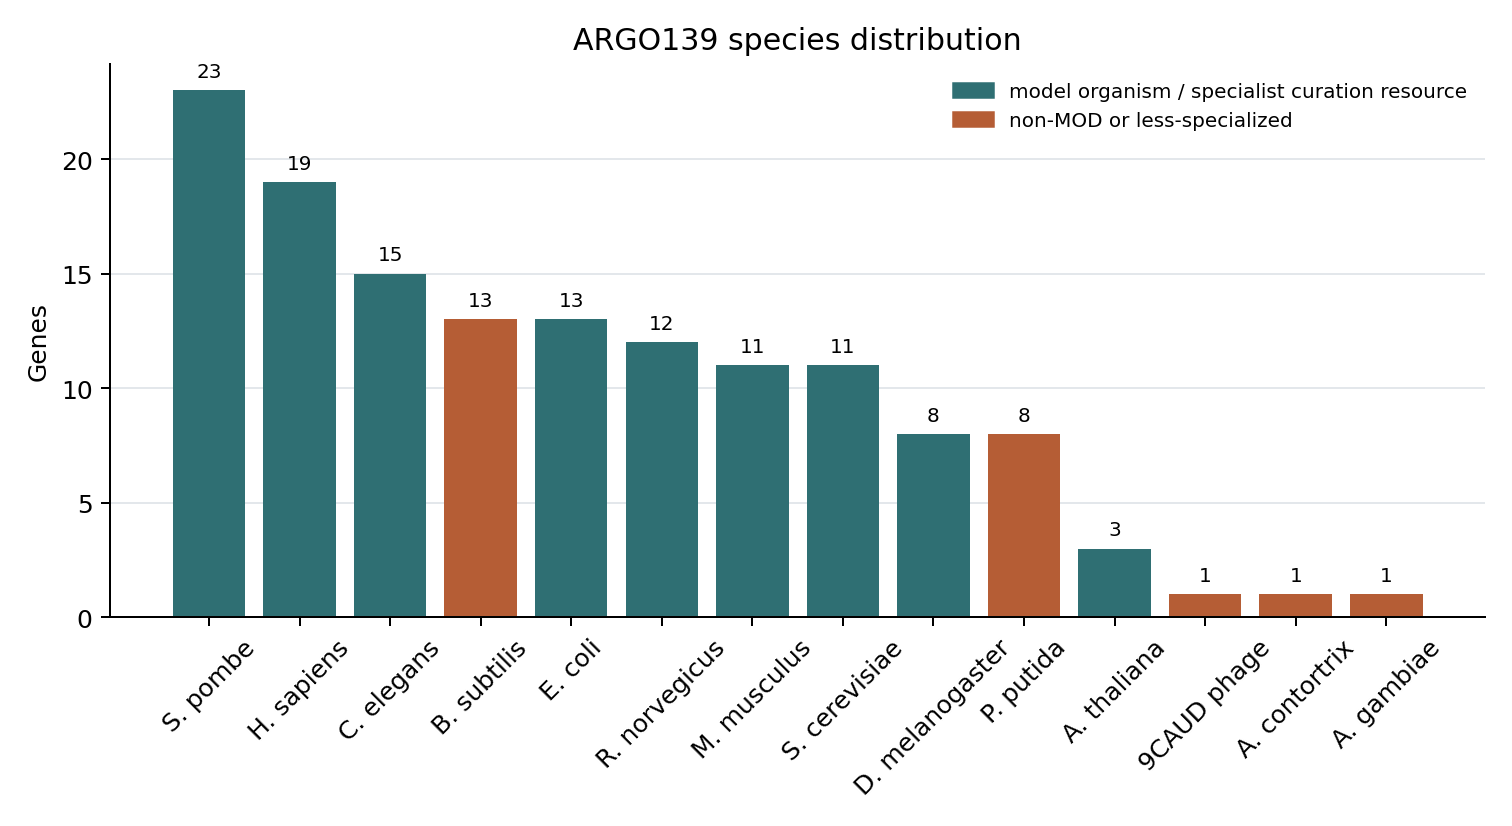
\includegraphics{figures/argo139_species_distribution.png}
\caption{ARGO139 species distribution. Teal bars mark model-organism or
specialist-resource species; orange bars mark non-MOD or
less-specialized species.}
\end{figure}

For each ARGO139 gene we obtained the BioReason-Pro RL functional
summary and reasoning trace from the public BioReason-Pro web
application (\texttt{app.bioreason.net}). We also ran the AI-AUGR pipeline
to produce an agent-adjudicated local reference review. These references
were not independently expert-signed: at the frozen audit baseline, 64/139
were \texttt{COMPLETE}, 48 \texttt{DRAFT}, 23 \texttt{IN\_PROGRESS}, and 4
\texttt{INITIALIZED}. A
dedicated \textbf{comparison agent} then scored each BioReason-Pro RL
output against the AI-AUGR review along two axes, each on a 1--5 scale:

\begin{itemize}
\tightlist
\item
  \textbf{Correctness}: 5 = all material claims supported; 4 = core function
  correct with one limited secondary error; 3 = core function correct but
  one or more substantive claims wrong; 2 = some relevant biology but errors
  materially distort the function; 1 = fundamental mischaracterisation.
\item
  \textbf{Completeness}: 5 = covers core functions, locations, complexes,
  and pathway context; 4 = core plus most major context with a limited
  omission; 3 = gets the basics but misses significant biology; 2 = only
  one important facet or substantially incomplete; 1 = superficial or
  misses the core function.
\end{itemize}

Omissions were charged to completeness rather than correctness. The
comparison agent wrote an evidence-based rationale and a qualitative
comparison against the supplied InterPro domain/family labels: does
BioReason-Pro add biological insight beyond those labels, or narratively
restate them? Only 92/139 genes had a \texttt{GO\_REF:0000002} annotation
in the committed GOA snapshot, so we treat actual InterPro2GO as a baseline
only for that subset. Reviews
were stored per gene as \texttt{\{GENE\}-bioreason-rl-review.md}, with
the raw BioReason-Pro export cached as
\texttt{\{GENE\}-bioreason-rl-predictions.md}.

ARGO139 is the collected export cohort, not the unconditional performance
denominator. We excluded \textbf{csr-1} from model-performance aggregates
because the supplied record and sequence were nhr-47/Q17370 rather than
CSR-1. Seven retained exports were exact 2,000-residue prefixes of longer
UniProt sequences (Dscam1, BRCA2, HTT, LRRK2, human and mouse NOTCH1, and
TOR1) and were flagged as sequence-truncated. The frozen policy and
per-gene manifest record export timestamps, expected and cached accessions,
sequence lengths, reference status, latest GOA annotation date, and SHA-256
checksums.

To measure score reproducibility, a second rater independently scored a
deterministic 20-gene subset. We balanced the sample by taking four genes
from each first-rater correctness stratum; within each stratum selection was
the SHA-256 order of a fixed release salt plus species/gene key. The second
rater could read only the raw RL export and local AIGR reference, not the
first review, project metrics, issue, or git history. We report exact and
within-one agreement, mean absolute error, Pearson and Spearman association,
and quadratic-weighted Cohen's kappa. This balanced design tests the full
rubric range rather than estimating prevalence-weighted ARGO139 agreement.

For SFT GO-term review we used only the public HuggingFace
\texttt{wanglab/protein\_catalogue} source. This defines ARGO95: the
95/139 ARGO139 genes present in that snapshot, with 955 SFT GO-term
predictions. We did not fill the remaining 44 ARGO139 genes from the
BioReason-Pro web export in the primary SFT analysis because that export
exposes a fundamentally different high-recall GO-term panel, including
many ancestor and obsolete terms. Web-export SFT terms, the SFT narrative
cross-check, and a separate GO-GPT overlap review are retained only as
supplemental material.

We also rebuilt the ARGO139 GO-GPT leaf files from the raw web exports.
Ontology-aware pruning retained 5,923 terms: 1,900 exact positive AIGR
matches (CNN), 129 exact rejected or over-annotated matches (NPI), and
3,894 unresolved terms (UNC). Documents with unresolved placeholders are
marked \texttt{DRAFT}; 138/139 therefore remain pending, and this set is not
reported as a completed GO-GPT performance evaluation.

\hypertarget{case-study-2-esr-ecoli-det-mini-recap}{%
\subsection{Case study 2: ESR-ECOLI-DET-Mini
recap}\label{case-study-2-esr-ecoli-det-mini-recap}}

From the 453 DeepECTransformer predictions in de Crécy-Lagard \emph{et
al.} \cite{decrecylagard2025} we selected 7 genes spanning all error classes represented
in the paper, specifically: \textbf{ygfF} (COR), \textbf{yciO} and
\textbf{yegV} (PLI), \textbf{yjhQ} and \textbf{yrhB} (NPI),
\textbf{yjdM} (UNC), and \textbf{fepE} (REP). This quick-check benchmark
is \texttt{ESR-ECOLI-DET-Mini} (alias \texttt{ESR-ECOLI-DET-7};
Zenodo dataset \cite{mungall2026esrecolidetmini}). Selection was
deterministic from the published tables and used the published classes. The current
repository artifacts are therefore not blinded: the project file lists
the paper's verdicts, the gene reviews can cite PMID:40703034, and the
structured prediction-review files quote the de Crécy-Lagard rationale
directly. We treat this exercise as a positive-control reproduction of
the taxonomy, not as an independent validation of AI-AUGR accuracy.

For each gene we ran the full AI-AUGR pipeline to produce a gene review,
and separately produced a \texttt{predictions-review.yaml} for the
DeepECTransformer prediction itself, using the same COR, CNN, LSP, PLI,
NPI, REP, and UNC taxonomy and structured error-type tags described in
§3.1. After review completion we compared the agent's classification
and rationale against the published classification in
\cite{decrecylagard2025}.

To probe how much of this result depends on label/rationale leakage, we
also archived an independent answer-key-withheld recapitulation
experiment. This run was performed on an ablated branch in which review
content was regenerated, and the reviewer reported that the de
Crécy-Lagard source paper, including PMID:40703034 and the published
rationales, was not used. The evidence package was not restricted to
curated annotations alone: it used UniProt, GOA, the DeepECTF paper,
primary literature, and one in-house bioinformatics analysis for yciO.
We therefore treat it as a literature- and bioinformatics-assisted
Expert Synthetic Review recap with the answer key withheld, not as a
strict curated-annotation-only benchmark. The result bundle is preserved
under
\texttt{projects/BIOREASON\_COMPARISON/recapitulation-experiment/claude-expt-1/};
all 7 copied gene reviews and all 7 copied prediction reviews validate
against the LinkML schema.

\hypertarget{reproducibility}{%
\subsection{Reproducibility}\label{reproducibility}}

All reviews, raw predictions, local AIGR references, and validator
configurations for both case studies are in the repository under
\texttt{genes/\{ORG\}/\{GENE\}/} and
\texttt{projects/BIOREASON\_COMPARISON/}. \texttt{genes.csv} is the
ARGO139 member list; \texttt{argo139-species-counts.csv},
\texttt{argo139-curation-context-counts.csv},
\texttt{benchmark-cohorts.csv}, and \texttt{benchmark-genes.csv}
enumerate the cohort composition and source provenance. The
GO hierarchy and ID-label audit use the official archived 2026-03-25
\texttt{go-basic.obo}; its SHA-256 is pinned in the benchmark policy and
release-specific active and obsolete sentinel terms are checked at load
time. GOA snapshots may retain identifiers after ontology obsoletion.
The
\texttt{ESR-ECOLI-DET-Mini} result bundle is archived on Zenodo
\cite{mungall2026esrecolidetmini}. Supplemental source-availability
details are in \url{supplemental-benchmark-details.md}. The repository
contains the scripts and configuration needed to reproduce each stage.
The full corpus of 139 BioReason-Pro reviews and 7 \emph{E. coli}
prediction reviews is also browsable at the public site.

\hypertarget{results}{%
\section{Results}\label{results}}

\hypertarget{the-ai-augr-recapitulates-major-expert-failure-calls-but-not-all-nuance}{%
\subsection{AI-AUGR recapitulates major expert failure calls but not
all
nuance}\label{the-ai-augr-recapitulates-major-expert-failure-calls-but-not-all-nuance}}

We first asked whether AI-AUGR can represent and apply an existing expert
biological-validity taxonomy before using it to evaluate BioReason-Pro.
In the original \texttt{ESR-ECOLI-DET-Mini} artifacts, all 7 AI-AUGR
prediction-review classifications matched the published de Crécy-Lagard
classifications and recorded substantially the same mechanistic
rationale (\textbf{Table 3}). Because the paper's labels and rationales
were available in those artifacts, this result is a positive control
rather than a blinded benchmark.

The answer-key-withheld recapitulation gives a more realistic estimate
of what an agentic synthetic reviewer can do. It recovered 4/7 exact
labels: fepE (REP), yciO (PLI), yjhQ (NPI), and yrhB (NPI). The misses
were biologically informative rather than random. For yegV and ygfF, the
reviewer chose UNC rather than the expert PLI/COR calls, reflecting
conservative uncertainty around substrate identity and in-vivo role. For
yjdM, the reviewer called NPI rather than UNC, over-converting an
in-vitro-versus-in-vivo ambiguity into a rejection. Thus the agent did
not reach the same level of expert nuance, but it did identify several
high-value smell-test failures: frequency-biased histidine-kinase
overprediction, paralog overannotation, and pathway-context violations.

\textbf{Table 3.} Positive-control reproduction and answer-key-withheld
recapitulation of de Crécy-Lagard \emph{et al.} \cite{decrecylagard2025} on 7 \emph{E.
coli} DeepECTransformer predictions.

\begin{longtable}[]{@{}lllll@{}}
\toprule
\begin{minipage}[b]{0.17\columnwidth}\raggedright
Gene\strut
\end{minipage} & \begin{minipage}[b]{0.17\columnwidth}\raggedright
Paper class\strut
\end{minipage} & \begin{minipage}[b]{0.17\columnwidth}\raggedright
Positive-control AI-AUGR class\strut
\end{minipage} & \begin{minipage}[b]{0.17\columnwidth}\raggedright
Answer-key-withheld class\strut
\end{minipage} & \begin{minipage}[b]{0.17\columnwidth}\raggedright
Interpretation\strut
\end{minipage}\tabularnewline
\midrule
\endhead
\begin{minipage}[t]{0.17\columnwidth}\raggedright
ygfF\strut
\end{minipage} & \begin{minipage}[t]{0.17\columnwidth}\raggedright
COR\strut
\end{minipage} & \begin{minipage}[t]{0.17\columnwidth}\raggedright
COR\strut
\end{minipage} & \begin{minipage}[t]{0.17\columnwidth}\raggedright
UNC\strut
\end{minipage} & \begin{minipage}[t]{0.17\columnwidth}\raggedright
Conservative miss; in-vitro SDR/glucose-DH evidence judged insufficient
for in-vivo function\strut
\end{minipage}\tabularnewline
\begin{minipage}[t]{0.17\columnwidth}\raggedright
yciO\strut
\end{minipage} & \begin{minipage}[t]{0.17\columnwidth}\raggedright
PLI\strut
\end{minipage} & \begin{minipage}[t]{0.17\columnwidth}\raggedright
PLI\strut
\end{minipage} & \begin{minipage}[t]{0.17\columnwidth}\raggedright
PLI\strut
\end{minipage} & \begin{minipage}[t]{0.17\columnwidth}\raggedright
Paralog-overannotation call recovered\strut
\end{minipage}\tabularnewline
\begin{minipage}[t]{0.17\columnwidth}\raggedright
yegV\strut
\end{minipage} & \begin{minipage}[t]{0.17\columnwidth}\raggedright
PLI\strut
\end{minipage} & \begin{minipage}[t]{0.17\columnwidth}\raggedright
PLI\strut
\end{minipage} & \begin{minipage}[t]{0.17\columnwidth}\raggedright
UNC\strut
\end{minipage} & \begin{minipage}[t]{0.17\columnwidth}\raggedright
Conservative miss around sugar-kinase substrate identity\strut
\end{minipage}\tabularnewline
\begin{minipage}[t]{0.17\columnwidth}\raggedright
yjhQ\strut
\end{minipage} & \begin{minipage}[t]{0.17\columnwidth}\raggedright
NPI\strut
\end{minipage} & \begin{minipage}[t]{0.17\columnwidth}\raggedright
NPI\strut
\end{minipage} & \begin{minipage}[t]{0.17\columnwidth}\raggedright
NPI\strut
\end{minipage} & \begin{minipage}[t]{0.17\columnwidth}\raggedright
Pathway-absence call recovered\strut
\end{minipage}\tabularnewline
\begin{minipage}[t]{0.17\columnwidth}\raggedright
yrhB\strut
\end{minipage} & \begin{minipage}[t]{0.17\columnwidth}\raggedright
NPI\strut
\end{minipage} & \begin{minipage}[t]{0.17\columnwidth}\raggedright
NPI\strut
\end{minipage} & \begin{minipage}[t]{0.17\columnwidth}\raggedright
NPI\strut
\end{minipage} & \begin{minipage}[t]{0.17\columnwidth}\raggedright
Wrong-enzyme/pathway-context call recovered\strut
\end{minipage}\tabularnewline
\begin{minipage}[t]{0.17\columnwidth}\raggedright
yjdM\strut
\end{minipage} & \begin{minipage}[t]{0.17\columnwidth}\raggedright
UNC\strut
\end{minipage} & \begin{minipage}[t]{0.17\columnwidth}\raggedright
UNC\strut
\end{minipage} & \begin{minipage}[t]{0.17\columnwidth}\raggedright
NPI\strut
\end{minipage} & \begin{minipage}[t]{0.17\columnwidth}\raggedright
Overcalled an in-vitro/in-vivo ambiguity as incorrect\strut
\end{minipage}\tabularnewline
\begin{minipage}[t]{0.17\columnwidth}\raggedright
fepE\strut
\end{minipage} & \begin{minipage}[t]{0.17\columnwidth}\raggedright
REP\strut
\end{minipage} & \begin{minipage}[t]{0.17\columnwidth}\raggedright
REP\strut
\end{minipage} & \begin{minipage}[t]{0.17\columnwidth}\raggedright
REP\strut
\end{minipage} & \begin{minipage}[t]{0.17\columnwidth}\raggedright
Frequency-bias histidine-kinase call recovered\strut
\end{minipage}\tabularnewline
\bottomrule
\end{longtable}

The recorded rationales are important, not just the class labels. In the
yciO case, both runs converged on a paralog-subfamily argument. In yjhQ
and yrhB, the withheld run recovered organism/pathway-context failures.
In fepE, it recognised the Wzz O-antigen length-regulator assignment and
the absence of a histidine-kinase domain. These are precisely the kinds
of triage signals a database team would want before spending expert time
on a large sequence-AI prediction set. The disagreements also set the
boundary: agentic review is useful for prioritising suspicious
predictions and detecting recurring error modes, but current outputs
should still be treated as curator-assistive rather than
curator-equivalent.

\hypertarget{argo95-sft-go-term-review}{%
\subsection{ARGO95 SFT GO-term
review}\label{argo95-sft-go-term-review}}

We next reviewed BioReason-Pro SFT GO-term predictions on ARGO95. Each
predicted term was classified against GOA and the AI-AUGR review using the
Expert Synthetic Review taxonomy: terms already in GOA were assigned
CNN; terms absent from GOA but supported by AI-AUGR core functions or
accepted annotations were reviewed as COR candidates; terms contradicted
by the AI-AUGR review were reviewed as NPI candidates; less precise terms
were assigned LSP; high-frequency generic terms were assigned REP; and
terms not supported or refuted by available evidence were assigned UNC.

ARGO95 uses the cleaner HuggingFace
\texttt{wanglab/protein\_catalogue} source: 95 ARGO139 genes and 955
terms. We exclude the web-export-only SFT terms from the primary
analysis because they expose a much larger GO ancestor hierarchy and are
not comparable to the HF catalogue term set. The web-export view remains
in the supplement as a source-diagnostic check, not as part of the main
SFT denominator.

\textbf{Table 4.} ARGO95 SFT GO-term assessment distribution.

\begin{longtable}[]{@{}rrrrrrrrr@{}}
\toprule
Genes & Terms & CNN & NPI & PLI & COR & LSP & REP & UNC\tabularnewline
\midrule
\endhead
95 & 955 & 658 (68.9\%) & 125 (13.1\%) & 5 (0.5\%) &
23 (2.4\%) & 61 (6.4\%) & 29 (3.0\%) & 54 (5.7\%)\tabularnewline
\bottomrule
\end{longtable}

\begin{figure}
\centering
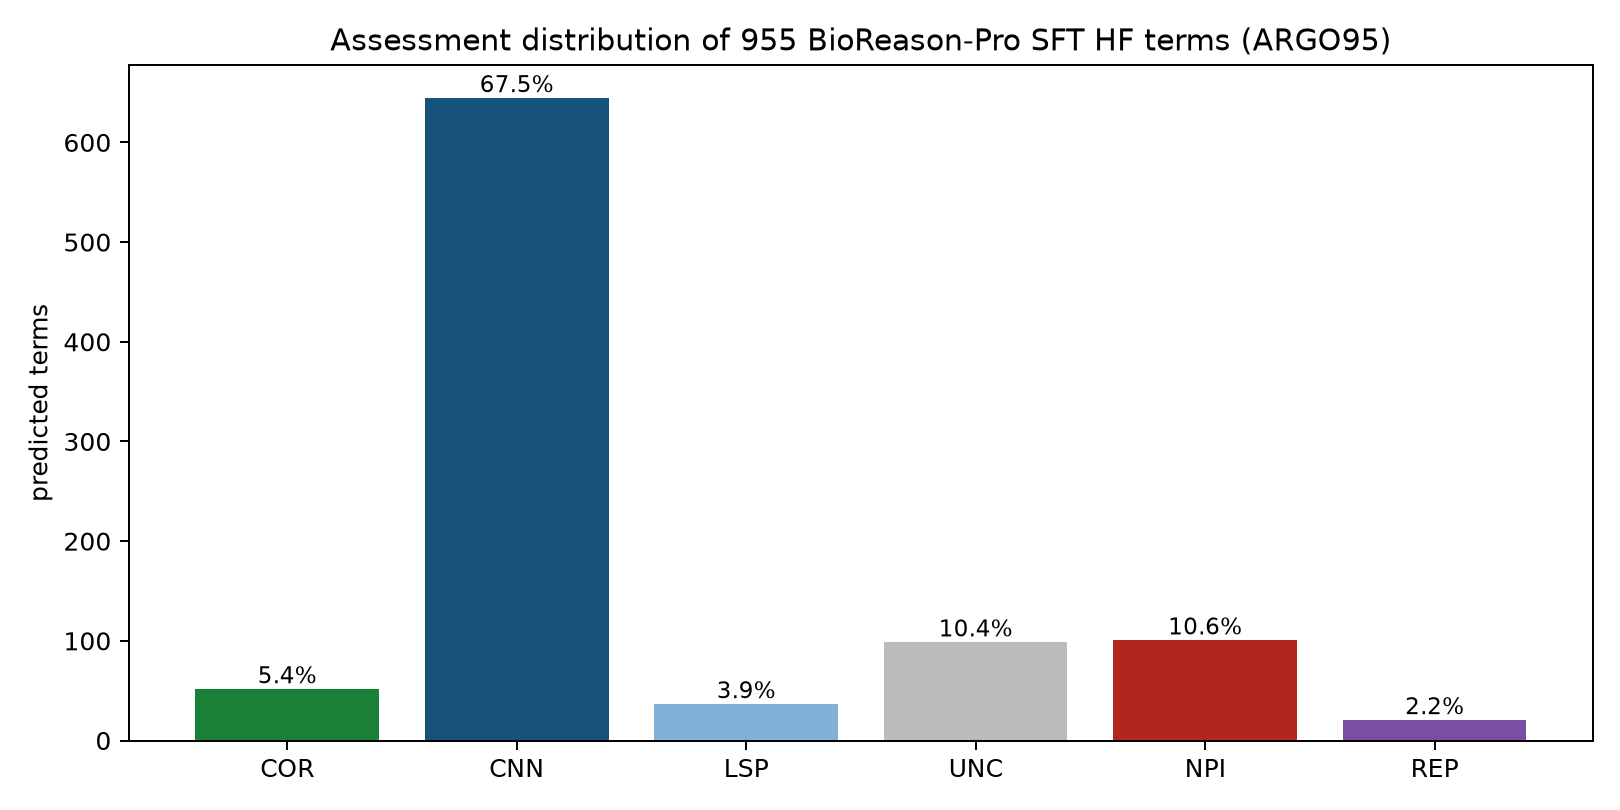
\includegraphics{figures/sft_assessment_distribution.png}
\caption{Assessment distribution for 955 BioReason-Pro SFT HF-catalogue
terms on ARGO95. CNN dominates; COR terms are known biology
absent from GOA, not functions unknown to the literature.}
\end{figure}

ARGO95 gives the cleanest estimate of SFT term quality: 658/955 (68.9\%)
of SFT terms are correct but non-novel, including 629 exact frozen-GOA
matches; 159/955 (16.6\%) are NPI, PLI, or REP; and only 23/955 (2.4\%)
are correct terms absent from frozen GOA that a database might
consider importing. The COR calls are not discoveries of biology unknown
to the literature. They are known functions missing from GOA or captured
less precisely than the model's term, such as RAS2 activation of
adenylate cyclase, Atg2 intermembrane lipid transfer, regulation of
mitochondrial gene expression by atfs-1, and the phosphatidylinositol
deacylase activity of bst1.

As a Tier-1 baseline, we also computed a retrospective CAFA-style
GOA-agreement score for the same SFT terms. Because BioReason-Pro SFT
terms are unranked, this is a single-threshold \(F_1\) rather than
\(F_{\max}\). After propagating predictions and current GOA annotations
over GO \texttt{is\_a} and \texttt{part\_of} ancestors, the HF subset
scored precision \(0.865\), recall \(0.479\), and \(F_1=0.617\) against
current GOA; exact-term \(F_1\) was \(0.418\). This makes the prediction
set look reasonably concordant with GOA, but the biological review shows
why agreement is not enough: 52/159 HF terms labelled NPI, PLI, or REP were
exact matches to current GOA, and 123/159 had propagated overlap with
current GOA. A CAFA-style score can therefore be a useful Tier-1
baseline, but it cannot distinguish restatement from novelty or current
database agreement from biological validity.

The excluded web-export subset makes a different point. Because it
contains many ancestor terms, even leaf filtering leaves a much larger
and more uncertain term panel than the HF catalogue. We therefore treat
web-export SFT terms as a supplemental source-availability diagnostic,
not as interchangeable observations in the ARGO95 SFT analysis.

The incorrect SFT terms recapitulate the same biological failure modes
seen in the RL narratives: pseudoenzyme overcalls, holdase/foldase
confusion in bacterial chaperones, wrong compartments,
antibiotic-target/response confusion, and substrate/partner role
reversal. The RAS2 and CpxP cases also show that the term and narrative
arms can fail independently. RAS2's SFT GO terms include the core
adenylate-cyclase activation biology that the RL narrative missed;
CpxP's SFT terms place it in the periplasm while the RL narrative calls
it cytoplasmic. For database deployment, neither output should be
trusted without reviewing the other.

\hypertarget{argo139-rl-narrative-review}{%
\subsection{ARGO139 RL narrative
review}\label{argo139-rl-narrative-review}}

Across the ARGO139 performance set (138/139 collected exports after the
wrong-input exclusion), BioReason-Pro RL achieved a mean correctness of
\textbf{4.0/5} and a mean completeness of \textbf{2.9/5} against the
agent-adjudicated local AIGR reference. The two axes are reported
separately; their empirical association was Pearson 0.688 and Spearman 0.617,
rather than the weak association asserted in the earlier analysis.
The score distribution
is shown in \textbf{Table 5}.

\textbf{Table 5.} Score distribution for BioReason-Pro RL on the 138-gene
ARGO139 performance set.

\begin{longtable}[]{@{}lrr@{}}
\toprule
Score & Correctness & Completeness\tabularnewline
\midrule
\endhead
5 & 70 (51\%) & 1 (1\%)\tabularnewline
4 & 25 (18\%) & 40 (29\%)\tabularnewline
3 & 22 (16\%) & 51 (37\%)\tabularnewline
2 & 14 (10\%) & 39 (28\%)\tabularnewline
1 & 7 (5\%) & 7 (5\%)\tabularnewline
\bottomrule
\end{longtable}

The high-correctness tail is real: 70 genes scored 5/5 on correctness.
But completeness is much weaker; only one gene scored 5/5 on both axes
(Uggt1, whose InterPro family name is itself highly diagnostic).

In the blinded 20-gene second review, correctness agreement was 80\% exact
and 100\% within one point (mean absolute error 0.20; quadratic-weighted
kappa 0.950). Completeness agreement was 55\% exact and 95\% within one
point (mean absolute error 0.50; kappa 0.744). Both axes matched exactly for
55\% of cases. The lower completeness agreement identifies coverage scoring
as the less reproducible judgment and supports reporting calibration data
alongside the aggregate means.
Mouse has the highest selected-case descriptive correctness mean (4.7),
followed by \emph{B. subtilis} (4.5), rat (4.4), and human (4.3), whereas
the selected \emph{S. pombe} cases have the lowest mean (3.2). This
comparison is confounded by
deliberate case mix: the \emph{S. pombe} set is enriched for obscure
proteins and pseudoenzymes, while the mammalian set contains more
canonical proteins. Training-distribution skew and InterPro-label
informativeness remain hypotheses rather than measured explanations.

\begin{figure}
\centering
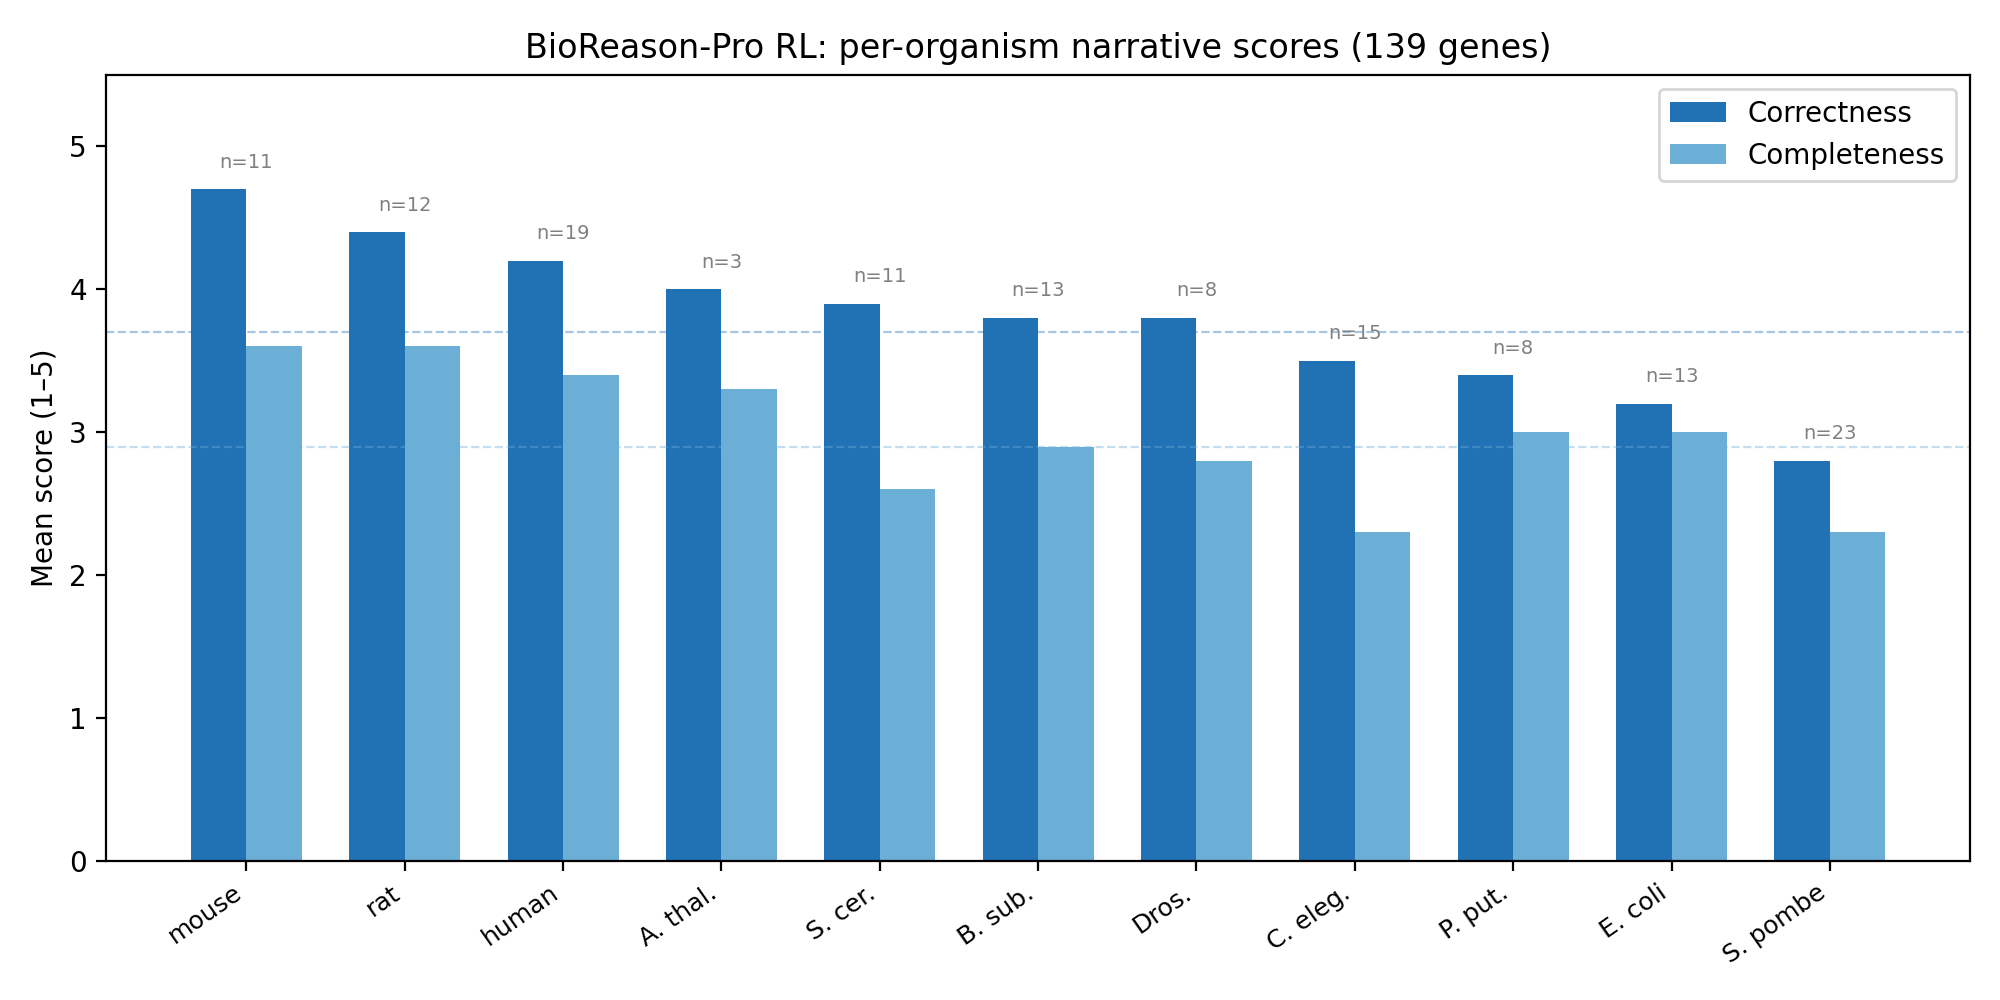
\includegraphics{figures/per_organism_scores.png}
\caption{Descriptive per-organism correctness and completeness for the
selected BioReason-Pro RL cases. Dashed lines show overall means and sample
size is shown above each bar pair. Uneven case selection precludes causal or
population-level interpretation.}
\end{figure}

The failures are not random. We identified eight reproducible model-output modes in
the RL narratives (\textbf{Table 6}). Recording them as error modes is
immediately useful for curation triage, because each points to a
specific missing capability: catalytic-residue checking, signal-peptide
and transmembrane reasoning, paralog-subfamily discrimination,
organism-context reasoning, and detection of training-set leakage.

\textbf{Table 6.} Representative ARGO139 RL narrative failure modes.

\begin{longtable}[]{@{}lll@{}}
\toprule
\begin{minipage}[b]{0.30\columnwidth}\raggedright
Failure mode\strut
\end{minipage} & \begin{minipage}[b]{0.30\columnwidth}\raggedright
Gene (organism)\strut
\end{minipage} & \begin{minipage}[b]{0.30\columnwidth}\raggedright
Brief description of the failure\strut
\end{minipage}\tabularnewline
\midrule
\endhead
\begin{minipage}[t]{0.30\columnwidth}\raggedright
Pseudoenzyme blind spot\strut
\end{minipage} & \begin{minipage}[t]{0.30\columnwidth}\raggedright
Epe1 (\emph{S. pombe})\strut
\end{minipage} & \begin{minipage}[t]{0.30\columnwidth}\raggedright
Claims JmjC demethylase activity despite degenerate active site and no
in-vitro activity\strut
\end{minipage}\tabularnewline
\begin{minipage}[t]{0.30\columnwidth}\raggedright
Pseudoenzyme blind spot\strut
\end{minipage} & \begin{minipage}[t]{0.30\columnwidth}\raggedright
cts2 (\emph{S. pombe})\strut
\end{minipage} & \begin{minipage}[t]{0.30\columnwidth}\raggedright
Called active chitinase despite lacking catalytic glutamate\strut
\end{minipage}\tabularnewline
\begin{minipage}[t]{0.30\columnwidth}\raggedright
Localisation default\strut
\end{minipage} & \begin{minipage}[t]{0.30\columnwidth}\raggedright
CpxP (\emph{E. coli})\strut
\end{minipage} & \begin{minipage}[t]{0.30\columnwidth}\raggedright
Called cytoplasmic; is periplasmic with a cleavable signal peptide\strut
\end{minipage}\tabularnewline
\begin{minipage}[t]{0.30\columnwidth}\raggedright
Localisation default\strut
\end{minipage} & \begin{minipage}[t]{0.30\columnwidth}\raggedright
ETR1 (\emph{A. thaliana})\strut
\end{minipage} & \begin{minipage}[t]{0.30\columnwidth}\raggedright
Called soluble cytoplasmic signal transducer; is an ER-membrane
receptor\strut
\end{minipage}\tabularnewline
\begin{minipage}[t]{0.30\columnwidth}\raggedright
Paralog indistinguishability\strut
\end{minipage} & \begin{minipage}[t]{0.30\columnwidth}\raggedright
Fyn / Src (mouse)\strut
\end{minipage} & \begin{minipage}[t]{0.30\columnwidth}\raggedright
Generic Src-family kinase descriptions; misses paralog-specific
biology\strut
\end{minipage}\tabularnewline
\begin{minipage}[t]{0.30\columnwidth}\raggedright
Paralog indistinguishability\strut
\end{minipage} & \begin{minipage}[t]{0.30\columnwidth}\raggedright
sigF/sigG/sigK (\emph{B. subtilis})\strut
\end{minipage} & \begin{minipage}[t]{0.30\columnwidth}\raggedright
Treated as generic sigma factors; compartment-stage sporulation biology
absent\strut
\end{minipage}\tabularnewline
\begin{minipage}[t]{0.30\columnwidth}\raggedright
Organism-specific biology absent\strut
\end{minipage} & \begin{minipage}[t]{0.30\columnwidth}\raggedright
daf-16 (\emph{C. elegans})\strut
\end{minipage} & \begin{minipage}[t]{0.30\columnwidth}\raggedright
Generic FoxO; no IIS/longevity/dauer biology\strut
\end{minipage}\tabularnewline
\begin{minipage}[t]{0.30\columnwidth}\raggedright
Organism-specific biology absent\strut
\end{minipage} & \begin{minipage}[t]{0.30\columnwidth}\raggedright
atfs-1 (\emph{C. elegans})\strut
\end{minipage} & \begin{minipage}[t]{0.30\columnwidth}\raggedright
Generic bZIP; misses UPRmt master regulator identity\strut
\end{minipage}\tabularnewline
\begin{minipage}[t]{0.30\columnwidth}\raggedright
Neo-functionalisation missed\strut
\end{minipage} & \begin{minipage}[t]{0.30\columnwidth}\raggedright
Nmnat (\emph{Drosophila})\strut
\end{minipage} & \begin{minipage}[t]{0.30\columnwidth}\raggedright
NAD biosynthesis enzyme; moonlighting neuroprotection role missed\strut
\end{minipage}\tabularnewline
\begin{minipage}[t]{0.30\columnwidth}\raggedright
Narrative/GO disconnect\strut
\end{minipage} & \begin{minipage}[t]{0.30\columnwidth}\raggedright
RidA (\emph{E. coli})\strut
\end{minipage} & \begin{minipage}[t]{0.30\columnwidth}\raggedright
Narrative mechanism mostly right; emitted term is generic
\texttt{protein\ binding}\strut
\end{minipage}\tabularnewline
\begin{minipage}[t]{0.30\columnwidth}\raggedright
Cross-kingdom fold bias\strut
\end{minipage} & \begin{minipage}[t]{0.30\columnwidth}\raggedright
aprE (\emph{B. subtilis})\strut
\end{minipage} & \begin{minipage}[t]{0.30\columnwidth}\raggedright
Subtilisin described with human hemostasis and blood-coagulation
processes\strut
\end{minipage}\tabularnewline
\begin{minipage}[t]{0.30\columnwidth}\raggedright
Cross-kingdom fold bias\strut
\end{minipage} & \begin{minipage}[t]{0.30\columnwidth}\raggedright
PGRPLB (\emph{A. gambiae})\strut
\end{minipage} & \begin{minipage}[t]{0.30\columnwidth}\raggedright
Mosquito protein described as a fruit-fly protein\strut
\end{minipage}\tabularnewline
\begin{minipage}[t]{0.30\columnwidth}\raggedright
Generated UniProt-style fabrication\strut
\end{minipage} & \begin{minipage}[t]{0.30\columnwidth}\raggedright
Slc5a1 (rat)\strut
\end{minipage} & \begin{minipage}[t]{0.30\columnwidth}\raggedright
Model-generated ``UniProt Summary'' claims steroid-sulfate transport;
the cached UniProt record describes glucose/galactose cotransport\strut
\end{minipage}\tabularnewline
\bottomrule
\end{longtable}

The comparison with supplied InterPro domain and family labels explains
why the aggregate scores are misleading. Across ARGO139 the dominant
mode is narrative restatement: BioReason-Pro translates those labels into
prose without adding new biology. It succeeds when domain architecture is
diagnostic (TOR1, NOTCH1, PTEN, EGFR, spo0A) and fails when the biology
depends on catalytic-site loss, lineage-specific context, paralog
identity, or compartmental signals not encoded in the family name. For
the 92/139 genes with an actual InterPro2GO annotation, that mapping
provides a separate baseline; where a mapping or supplied family label is
wrong or uninformative, BioReason-Pro usually repeats the problem rather
than repairing it.

\hypertarget{discussion}{%
\section{Discussion}\label{discussion}}

\hypertarget{what-agentic-review-adds}{%
\subsection{What agentic review
adds}\label{what-agentic-review-adds}}

Agentic review surfaces information absent from aggregate scores, and
this information is what annotation database leads need for deployment
decisions.

First, it can read the narrative. BioReason-Pro emits free-text
summaries and reasoning traces whose scientific content cannot be
projected onto a bag of GO terms. AI-AUGR can grade those claims directly
against cached literature and existing annotation.

Second, it surfaces reproducible failure modes. In the ARGO139 performance
set, the RL mean correctness of 4.0/5 hides failures that are biologically patterned:
pseudoenzyme overcalls, localisation defaults, paralog
indistinguishability, missing organism-specific biology, missed
neo-functionalisation, narrative/GO disagreement, and cross-kingdom
bias. These are not merely lower scores; they are deployment warnings.

Third, it distinguishes novelty from restatement. The SFT GO-term review
shows that most terms are CNN, not new biology. The COR terms are useful
curation candidates, but they are known functions absent from GOA, not
discoveries unknown to the literature. A CAFA-style agreement score
cannot make that distinction.

\hypertarget{why-argo139}{%
\subsection{Why ARGO139}\label{why-argo139}}

The earlier draft separated the RL narrative, SFT term, and GO-GPT
overlap analyses into different denominators. That made the story
unnecessarily fragile. The current analysis uses ARGO139 as the fixed
biological gene set for RL narrative review and ARGO95 as the HF-only
SFT term subset nested inside ARGO139.

ARGO139 is still not a population sample. It was deliberately
constructed to span characterized biology, model-organism resources, and
non-MOD or less-specialized contexts such as \emph{B. subtilis}. That
design is appropriate for deployment triage because it enriches for the
edge cases where production databases most need review: pseudoenzymes,
paralogs, lineage-specific biology, compartments, and moonlighting
proteins. It should not be interpreted as an estimate of BioReason-Pro
performance on a random UniProt draw.

The main remaining complexity is source availability. The HuggingFace
SFT snapshot contains 95/139 ARGO139 genes; the remaining 44 can only be
filled from a web export that exposes a different, ancestor-rich term
panel. We therefore use ARGO95 for primary SFT term review and keep the
larger source-availability views and GO-GPT overlap review in the
supplement rather than in the main denominator story.

\hypertarget{esr-as-a-positive-control-and-recapitulation-stress-test}{%
\subsection{ESR as a positive control and recapitulation stress
test}\label{esr-as-a-positive-control-and-recapitulation-stress-test}}

A natural concern is that an LLM curator-agent might share failure modes
with the predictor it evaluates. The \texttt{ESR-ECOLI-DET-Mini}
positive-control exercise does not eliminate that concern, because it
was not blinded. Its value is narrower: it shows that AI-AUGR can encode
the same expert taxonomy and assemble the same kinds of mechanistic
rationale for pathway-presence reasoning, paralog-subfamily reasoning,
in-vitro/in-vivo distinction, and training-label-frequency-bias
detection.

The answer-key-withheld recapitulation narrows this concern but does not
remove it. Recovering 4/7 exact labels is not expert equivalence; the
agent was conservative on ygfF and yegV and too severe on yjdM. But the
run recovered the most operationally important incorrect-call patterns.
For deployment triage, this is the relevant signal. A database team does
not need an agent to be a final arbiter to benefit from it; it needs the
agent to flag suspicious sequence-AI outputs, identify the likely
failure mode, and route the case to a human curator with a traceable
rationale. A true external-validity test still requires a fresh blinded
set whose labels and rationales are withheld from both the evidence
package and the reviewing agent.

\hypertarget{three-tiers-of-function-prediction-evaluation}{%
\subsection{Three tiers of function-prediction
evaluation}\label{three-tiers-of-function-prediction-evaluation}}

It is useful to separate function-prediction evaluation into three
tiers.

\textbf{Tier 1: aggregate metric evaluation.} CAFA-style \(F_{\max}\)
and \(S_{\min}\) scale to large holdouts and enable method comparison,
but they inherit GOA-as-ground-truth bias, metric bias toward generic
terms, and do not directly grade narratives.

\textbf{Tier 2: expert or agentic biological-validity review.} A domain
expert, or an LLM curator-agent grounded in primary evidence, reads the
prediction and classifies it using a biological taxonomy such as
COR/CNN/LSP/NPI/REP/UNC. This is the tier AI-AUGR partially automates. It
is the right level for deployment decisions.

\textbf{Tier 3: prospective experimental validation.} This is the
strongest evidence but the least scalable. Protein function is
multi-dimensional: validating MF, BP, and CC claims can require
different assays, organisms, and conditions. Tier 3 is essential for
discovery claims, but not a practical first-pass filter for every
computational prediction.

\hypertarget{what-we-learned-about-bioreason-pro}{%
\subsection{What we learned about
BioReason-Pro}\label{what-we-learned-about-bioreason-pro}}

BioReason-Pro is not ready for unsupervised import into a production
annotation database. On ARGO95, its SFT terms mostly restate GOA, with
a non-trivial incorrect fraction in the cleaner HF subset. Its RL
narratives are often plausible prose versions of supplied InterPro
domain and family labels, not independent biological reasoning. The model
is useful when domain architecture is diagnostic, but fails when the answer depends on
catalytic-site loss, organism context, paralog identity, or
compartmental signals.

The model's best contribution may be format rather than current
accuracy. A narrative can be reviewed, corrected, and triaged in ways
that a naked GO-term list cannot. But the narrative and term arms must
be reviewed independently, because they can disagree.

\hypertarget{limitations}{%
\section{Limitations}\label{limitations}}

\textbf{Agent bias.} AI-AUGR itself depends on an LLM curator-agent. We
mitigate this through cached evidence, literal-quote checking, and
schema validation, but shared blind spots remain possible. The current
\texttt{ESR-ECOLI-DET-Mini} reproduction is useful as a positive
control, not as a blinded external validation. The answer-key-withheld
recapitulation is more informative, but its 4/7 exact-label result shows
that the agent still lacks expert-level boundary judgment.

\textbf{ARGO139 sample selection.} ARGO139 is manually selected for
characterized biology and hard deployment cases. It is not random, and
its estimates should not be read as population-level BioReason-Pro
performance.

\textbf{SFT subset availability.} ARGO95 covers the 95/139 ARGO139 genes
available in the HF catalogue. The remaining 44 genes can be represented
only by web-export SFT terms, but those terms include ancestor and
obsolete-term inflation and are therefore treated as a supplemental
source diagnostic rather than primary SFT observations.

\textbf{Rubric subjectivity.} The 1-5 Correctness and Completeness
scales involve judgement. We mitigate this by requiring supporting
evidence and releasing the per-gene reviews for inspection. A blinded
20-gene second review found higher reproducibility for correctness
(quadratic-weighted kappa 0.950) than completeness (0.744). A larger,
prevalence-weighted multi-rater study remains future work.

\textbf{Single predictor in depth.} We evaluate BioReason-Pro in detail,
plus DeepECTransformer through the \texttt{ESR-ECOLI-DET-Mini}
positive-control reproduction. Comparative evaluation across multiple
reasoner-style systems is out of scope.

\textbf{Label leakage and small recapitulation set.} The original 7-gene
\texttt{ESR-ECOLI-DET-Mini} exercise was selected from the published
tables and the repository artifacts include the published labels and
rationales. It should not be described as blinded. The archived
answer-key-withheld recapitulation removes the most direct leakage
source, but it is still small, selected after the de Crécy-Lagard study
was known, and literature/bioinformatics-assisted rather than a locked
curated-annotation-only benchmark. A stronger follow-up would hold out
the expert labels, remove PMID:40703034 from the per-gene evidence
package, pre-register the evidence mode, and score the agent's
classifications before unblinding.

\textbf{Reference-review staleness.} The agent-adjudicated local AIGR
references can become stale as literature and curation standards evolve.
The pipeline is reproducible, and the browse site exposes generated review files for
future reruns.

\hypertarget{conclusions}{%
\section{Conclusions}\label{conclusions}}

AI-AUGR reproduces the Expert Synthetic Review taxonomy on the 7-gene
\texttt{ESR-ECOLI-DET-Mini} positive-control set, showing that the
schema and review workflow can encode biologically meaningful error
classes. In an answer-key-withheld recapitulation, it recovered 4/7
exact expert labels and the main high-value incorrect-call patterns, but
not all expert boundary judgments. Applying AI-AUGR to ARGO139 shows that
BioReason-Pro mostly restates existing annotation pipelines,
occasionally names known biology missing from GOA, and makes systematic
errors that aggregate metrics would hide.

The practical conclusion is not that CAFA-style metrics should be
abandoned. It is that deployment decisions need a Tier 2 layer: expert
or agentic review that can read narratives, classify novelty, and
identify biologically meaningful failure modes. Agentic review is not
yet a human-curator replacement, but it is already useful as a scalable
smell test for sequence-AI predictions. ARGO139 and ARGO95 are our first
linked benchmarks for that layer across BioReason-Pro RL narratives and
SFT terms.

\hypertarget{figures}{%
\section{Figures}\label{figures}}

Figures are embedded inline. Additional planned figures for final
submission:

\begin{itemize}
\tightlist
\item
  \textbf{AI-AUGR pipeline diagram.} Evidence assembly (UniProt, GOA,
  InterPro, cached literature, deep-research report) → curator-agent
  three-phase review → LinkML validation → structured output. \emph{(To
  be created as a schematic.)}
\item
  \textbf{CAFA evaluation context.} For representative CAFA \(F_{\max}\)
  curves illustrating the aggregate evaluation paradigm, see Figure 2 of
  Radivojac \emph{et al.} \cite{radivojac2013} and Figure 1 of Zhou \emph{et al.}
  \cite{zhou2019}. Our work addresses the gap between such aggregate curves and
  the per-protein biological validity that deployment decisions require.
\end{itemize}

\hypertarget{data-and-code-availability}{%
\section{Data and code
availability}\label{data-and-code-availability}}

\emph{Repository:} \texttt{github.com/ai4curation/ai-gene-review} ---
ARGO139 BioReason-Pro RL narrative reviews and ARGO95 SFT GO-term reviews,
\texttt{article/supplemental-benchmark-details.md},
\texttt{ESR-ECOLI-DET-Mini} 7-gene \emph{E. coli} positive-control
reproduction and archived answer-key-withheld recapitulation results in
\texttt{projects/BIOREASON\_COMPARISON/recapitulation-experiment/claude-expt-1/},
archived on Zenodo \cite{mungall2026esrecolidetmini}, AI-AUGR pipeline,
LinkML schema, and validator.

\emph{Browsable reviews:}
\url{https://ai4curation.io/ai-gene-review/}

\bibliographystyle{unsrtnat}
\bibliography{references}

\end{document}
